%\documentclass[a4paper,handout]{beamer}
\documentclass[presentation]{beamer}
%\usepackage[francais]{babel}
\usepackage[utf8]{inputenc}
\usetheme{Inuits}
\usepackage[T1]{fontenc}
\usepackage{listings}
\usepackage{eso-pic}
\setbeamercolor{background canvas}{bg=} 
\definecolor{inuitstitle}{RGB}{153,153,255}
\definecolor{inuitsgreen}{RGB}{35,255,35}
\usecolortheme[RGB={90,90,149}]{structure} 
\usebackgroundtemplate{%

\includegraphics[height=\paperheight,widht=\paperwidth]{files/background.png};}

%\AddToShipoutPicture{\put(0,5){%
%   \parbox[b][\paperheight]{\paperwidth}{%
%     \vfill
%     \centering
%     \rotatebox{0}{
\includegraphics[width=\paperwidth,height=\paperheight,%
%                      ]{files/background.png}}%
%     \vfill
%}}}
\setbeamercolor{normal text}{fg=white}
\setbeamercolor{block body}{fg=black}
\setbeamercolor{itemize item}{fg=inuitsgreen}
\setbeamercolor{itemize subitem}{fg=inuitsgreen}
\setbeamercolor{itemize subitem subitem}{fg=inuitsgreen}
\setbeamertemplate{itemize item}[circle] 
\setbeamertemplate{itemize subitem}[circle] 
\setbeamertemplate{sections/subsections in toc}[circle]

%\setbeamercolor{palette primary}{fg=inuitstitle,bg=black!85}
%\setbeamercolor{palette secondary}{fg=white,bg=inuitstitle}
%\setbeamercolor{palette tertiary}{fg=white,bg=black!85}
%\setbeamercolor{palette quaternary}{fg=inuitstitle}
%\setbeamercolor{block title}{fg=inuitstitle}
%\setbeamercolor{sidebar}{bg=inuitstitle!70}

%\AtBeginDocument{%
%    \pgfdeclareverticalshading{beamer@topshade}{\paperwidth}{%
%      color(0pt)=(bg);
%      color(4pt)=(black)}
%}


\setbeamercolor{title}{fg=inuitstitle,bg=}

\setbeamertemplate{navigation symbols}{}
\definecolor{OliveGreen}{RGB}{0,100,0}
\definecolor{grey}{RGB}{150,150,150}
\definecolor{darkgrey}{RGB}{100,100,100}
\definecolor{inuits}{RGB}{153,153,255}
\usepackage{shadowtext}
\newcommand{\xitem}[1]{\item{\shadowtext{#1}}}
\newcommand{\inuits}[1]{\shadowtext{\color{inuits}#1}}

\newcommand{\ptitle}{Logstash and friends}

\begin{document}
\setbeamercovered{invisible}

\title[\ptitle]{\fontsize{25}{35}\selectfont \shadowtext{\ptitle}}

\author[Julien Pivotto]{\shadowtext{Julien Pivotto}}
%\institute[Inuits]{Inuits}
\date{\shadowtext{Techies Teach Techies}\\\inuits{September 2, 2013}}
\logo{
\includegraphics[height=2cm]{files/logstash2.png}}

\frame[plain,t]{\vspace{-1em} \centerline{
\includegraphics[width=\paperwidth]{files/loup.jpg}}\titlepage}
\frame{\tableofcontents}
\section{Introduction}
%\frame{%
%    \begin{center}\begin{Huge}{\inuits{Julien Pivotto}}\end{Huge}\end{center}
%    \begin{large}
%    \begin{itemize}
%        \xitem{sysadmin @ inuits}
%        \xitem{open-source defender for 7+ years}
%        \xitem{devops believer}
%        \xitem{@roidelapluie on twitter/github}
%    \end{itemize}
%    \end{large}
%}

%\subsection{Automation}
%\frame{%
%\frametitle{Infrastructure as Code}
%    \begin{LARGE}
%    \begin{itemize}
%        \xitem{Keep your environments under SCM}
%        \xitem{Overview of complete environments}
%        \xitem{Reduce the deployment time}
%    \end{itemize}
%    \end{LARGE}
%}
%\frame{%
%\frametitle{Keep all environments the same}
%
%    \flushright{\tiny{\color{darkgrey}http://www.flickr.com/photos/bobvietnam/4828291896/}}
%    \begin{center}
%        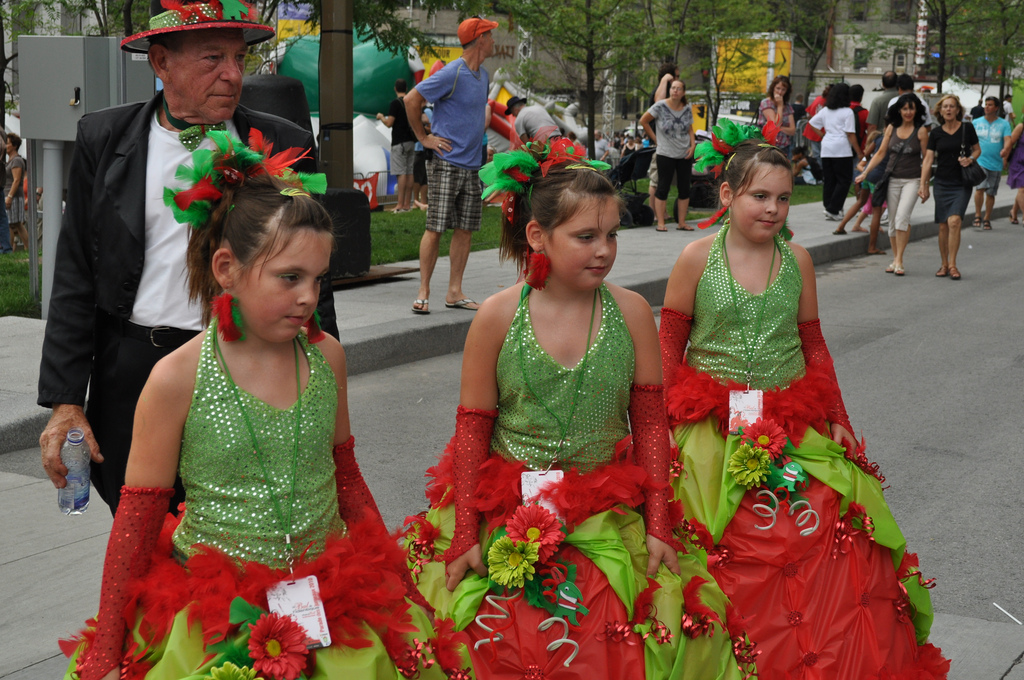
\includegraphics[height=6cm]{files/flickr_jumeaux.jpg}\\
%    \end{center}
%}

\frame{%
\frametitle{Logging}
\begin{itemize}
\xitem{Recording of events}
\xitem{Voice of your systems and applications}
\xitem{It tells you almose everything}
\xitem{It is a source of knowledge}
\end{itemize}
}
\frame{%
\frametitle{Logging is useful}
\begin{itemize}
\xitem{Understanding outages}\pause
\xitem{not only when it's wrong}
\xitem{you can extract metrics}
\xitem{no logs means something}
\xitem{it tells you what, why, who, when}
\end{itemize}
}
\frame{%
\frametitle{Logging in the wild}
\begin{itemize}
\xitem{Syslog}
\xitem{\texttt{|tee /var/log/myapp.log}}
\xitem{Cron + \texttt{MAILTO=}}
\xitem{\texttt{\&>/dev/null}}
\end{itemize}
}
\frame{%
\frametitle{Logging in the past}
\begin{itemize}
\xitem{Logging to files on each server}
\xitem{Using syslog protocol}
\xitem{Decentralized}
\xitem{Reading requires SSH access}
\xitem{Not developer friendly}
\end{itemize}
}
\frame{%
\frametitle{The tools nowadays}
\begin{itemize}
\xitem{Jenkins, Icinga, Graphite, Foreman}
\xitem{Nice web interfaces}
\xitem{Centralized}
\xitem{Easy to use}
\end{itemize}
}
\frame{%
\frametitle{Requirements}
\begin{itemize}
\xitem{Scalable tools}
\xitem{Configured by text files}
\xitem{Playing with existing tools}
\xitem{Scalable}
\xitem{Following the Unix philosophy}
\end{itemize}
}
\frame{%
\frametitle{3 separate tools}
\begin{itemize}
\xitem{Elasicsearch, distributed search \& analytics engine}
\xitem{Logstash, logs managment}
\xitem{Kibana, very nice webui to ES and Logstash}
\end{itemize}
}
\section{Logstash}
\frame{%
\frametitle{Logstash}
    \begin{center}
        
\includegraphics[height=7.5cm]{files/logstash.png}\\
    \end{center}
}
\subsection{Missions}
\frame{%
\frametitle{Shipping the logs}
\begin{itemize}
\xitem{Some applications can only write to files}
\xitem{But you need them on the main logstash server}
\xitem{Logstash can act as a daemon to ship the logs}
\xitem{Destinations can be syslog, redis,\ldots}
\xitem{Then you can act on your logs}
\end{itemize}
}
\frame{%
\frametitle{Collecting the logs}
\begin{itemize}
\xitem{You can plug logstash to a lot of data sources}
\xitem{It can be passive or active}
\xitem{Listening on a UDP port vs checking mails}
\xitem{All your logs are managed by one application}
\xitem{It creates fields from the logs}
\end{itemize}
}
\frame{%
\frametitle{Filtering the logs}
\begin{itemize}
\xitem{Making sense of a log message}
\xitem{Finding what is important}
\xitem{Adding and removing fields}
\end{itemize}
}
\frame{%
\frametitle{Storing the logs}
\begin{itemize}
\xitem{Output to Elasticsearch}
\xitem{Sending information to statsd}
\xitem{Sending to your inbox, to icinga or files}
\end{itemize}
}
\subsection{Inputs}
\frame{%
    \flushright{\tiny{\color{darkgrey}http://www.flickr.com/photos/quinnanya/7237788632/}}
    \begin{center}
        
\includegraphics[height=7cm]{files/eat.jpg}\\
    \end{center}
}
\frame{%
\frametitle{UDP and TCP input}
\begin{itemize}
\xitem{Compatible with rsyslog protocol}
\xitem{Each syslog talks with logstash directly}
\xitem{Allow you to use the syslog toolchains: logger, rsyslog}
\xitem{UDP is shoot and forget}
\end{itemize}
}
\begin{frame}[fragile]
\frametitle{UDP and TCP input}
\begin{block}{Logstash configuration}
\begin{verbatim}
input {
    udp {
        type => syslog
        port => 5544
    }
    tcp {
        type => syslog
        port => 5544
    }
}
\end{verbatim}
\end{block}
\end{frame}
\begin{frame}[fragile]
\frametitle{UDP and TCP input}
\begin{block}{Rsyslog configuration}
\begin{verbatim}
*.* @logstash.example.com:5544
\end{verbatim}
\end{block}
\begin{itemize}
\xitem In \texttt{/etc/rsyslog.conf}
\xitem That line will forward all the logs to logstash
\xitem Logstash will make useful fields out of it: priority, severity, program\dots
\end{itemize}
\end{frame}
\frame{%
\frametitle{File}
\begin{itemize}
\xitem{Enable you to use logstash with every application}
\xitem{Useful to ship the logs}
\xitem{Acts as a \texttt{tail -n 0 -F}}
\xitem{It works even if you use logrotate}
\end{itemize}
}
\begin{frame}[fragile]
\frametitle{File}
\begin{block}{}
\begin{verbatim}
input {
    file {
        path => "/var/log/legacyapp.log"
        type => "legacylog"
    }
}
\end{verbatim}
\end{block}
\end{frame}
\subsection{Filters}
\frame{%
\frametitle{Grok}
\begin{itemize}
\xitem{Extract fields from text}
\xitem{Useful to read messages}
\xitem{A lot of pre-existing patterns}
\xitem{Uses Regex to find out fields}
\end{itemize}
}
\begin{frame}[fragile]
\frametitle{Grok}
\begin{block}{Input text}
\begin{verbatim}
Invalid user oracle from 85.249.144.18
\end{verbatim}
\end{block}
\begin{block}{Grok pattern}
\begin{verbatim}
Invalid user %{USERNAME:login} from %{IP:ip}
\end{verbatim}
\end{block}
\begin{block}{Result}
\begin{verbatim}
{
    "login": [
        [ "oracle" ]
    ],
    "ip": [
        [ "85.249.144.18" ]
    ]
}
\end{verbatim}
\end{block}
\end{frame}
\begin{frame}[fragile]
\frametitle{Grok}
\begin{block}{}
\begin{small}
\begin{verbatim}
filter {
    grok {
        type    => "syslog"
        pattern => ["(?m)<%{POSINT:syslog_pri}>..."
        add_field => [ "received_at", "%{@timestamp}" ]
        add_field => [ "received_from", "%{@source_host}" ]
        add_tag  => "syslog-%{syslog_program}"
    }
}
\end{verbatim}
\end{small}
\end{block}
\end{frame}
\frame{%
\frametitle{Grep}
\begin{itemize}
\xitem{Allows you to grep interresting messages}
\xitem{Useful to count}
\end{itemize}
}
\begin{frame}[fragile]
\frametitle{Grep}
\begin{block}{}
\begin{small}
\begin{verbatim}
filter {
    grep {
        add_field => ["outputirc", "A puppet package
                                    has been deployed"]
        add_tag => "outputirc"
        drop => false
        match => [ "syslog_program", "yum" ]
        match => [ "@source_host", "puppetmaster" ]
        match => [ "@message", "puppet-tree" ]
    }
}
\end{verbatim}
\end{small}
\end{block}
\end{frame}
\begin{frame}[fragile]
\frametitle{Geoip}
\begin{block}{}
\begin{verbatim}
filter{
    geoip {
        tags   => ["syslog-httpd"]
        source => ["client"]
    }
}
\end{verbatim}
\end{block}
\begin{itemize}
\xitem{Transform ip address into geo data}
\xitem{Useful to filter by country/map the data}
\end{itemize}
\end{frame}
\subsection{Output}
\begin{frame}[fragile]
\frametitle{Elasticsearch}
\begin{itemize}
\xitem{Version of elasticsearch <=> version of logstash}
\xitem{Unless you use the elasticsearch\_http output}
\end{itemize}
\begin{block}{}
\begin{verbatim}
output {
    elasticsearch  {
    }
}
\end{verbatim}
\end{block}
\end{frame}
\begin{frame}[fragile]
\frametitle{IRC}
\begin{block}{}
\begin{verbatim}
output {
    irc {
        channels => ["#example"]
        host => "chat.freenode.net"
        nick => "loggy"
        port => 6667
        tags => "outputirc"
        user => "loggy"
        format => "%{outputirc}"  
    }
}
\end{verbatim}
\end{block}
\end{frame}
\section{Kibana}
\begin{frame}[fragile]
\frametitle{statsd}
\begin{block}{}
\begin{small}
\begin{verbatim}
output {
  statsd {
    host => '127.0.0.1'
    sender => "logstash"
    increment => [ "httpd.%{http_host}.r.%{response}",
                   "httpd.response.%{response}"]
    count => ["apache.%{http_host}.bytes", "%{bytes}" ]
    timing => ["apache.%{http_host}", "%{duration_msec}"]
    tags => 'grokked-apache'
  }
}
\end{verbatim}
\end{small}
\end{block}
\end{frame}
\frame{%
\frametitle{Kibana}
\begin{itemize}
\xitem{Kibana is a web interface for Logstash/ES}
\xitem{Kibana 1 was written in PHP}
\xitem{Kibana 2 was written in Ruby}
\xitem{Kibana 3 is written in AngularJS}
\end{itemize}
}
\frame{%
\frametitle{Kibana 3}
\begin{itemize}
\xitem{Everything happens in the browser}
\xitem{The browser is connected to Elasticsearch}
\xitem{You can save dashboards into ES}
\xitem{You can write/template dashboards to files}
\end{itemize}
}
\begin{frame}[fragile]
\frametitle{Installing kibana3}
\begin{block}{}
\begin{tiny}
\begin{verbatim}
git clone https://github.com/elasticsearch/kibana.git
ssh -NL 9200:127.0.0.1:9200 elasticsearch &
python -m SimpleHTTPServer
\end{verbatim}
\end{tiny}
\end{block}
\end{frame}
\begin{frame}[fragile]
\frametitle{Kibana queries}
\begin{block}{Example of a kibana query}
\begin{tiny}
\begin{verbatim}
@fields.syslog_program:"httpd" AND @fields.http_host:"test.example.com" AND @fields.response:"404"
\end{verbatim}
\end{tiny}
\end{block}
\begin{itemize}
\xitem Lucene query syntax
\xitem Simple and effective
\xitem Point \& click web interface
\end{itemize}
\end{frame}

\frame{%
\frametitle{Kibana}
    \begin{center}
        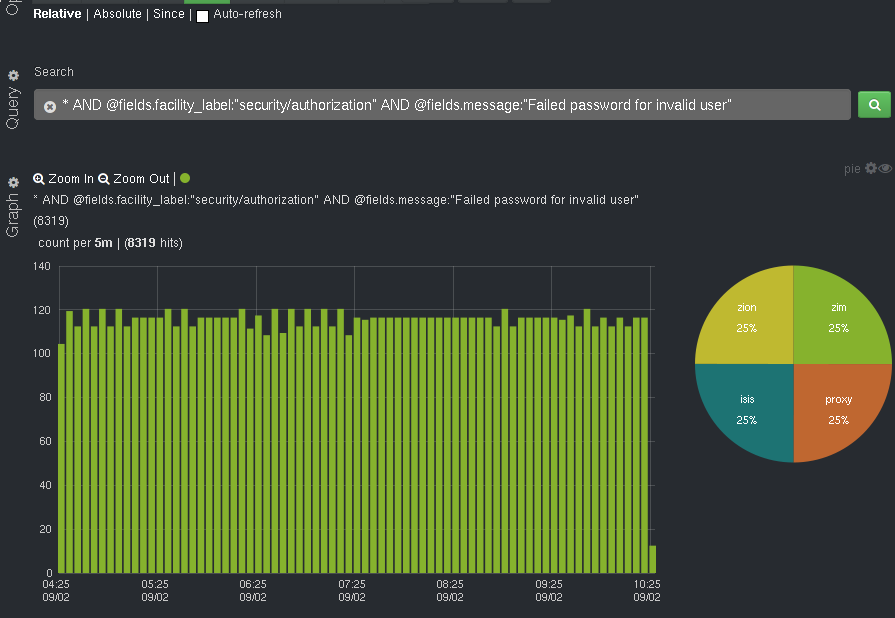
\includegraphics[height=7.5cm]{files/kibana3.png}\\
    \end{center}
}
\frame{%
\frametitle{Kibana}
    \begin{center}
        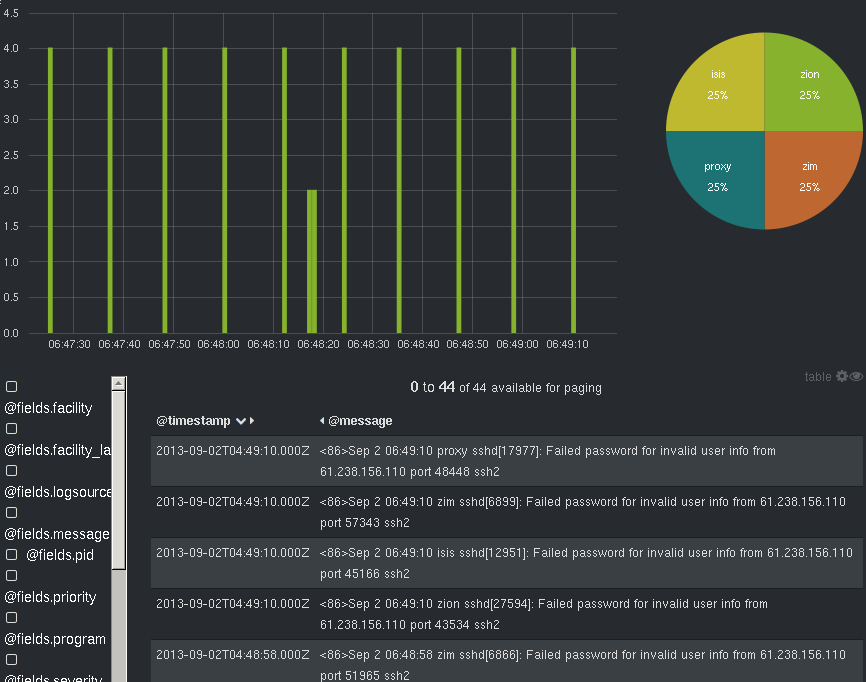
\includegraphics[height=7.5cm]{files/kibana3b.png}\\
    \end{center}
}
\frame{%
\frametitle{Kibana}
    \begin{center}
        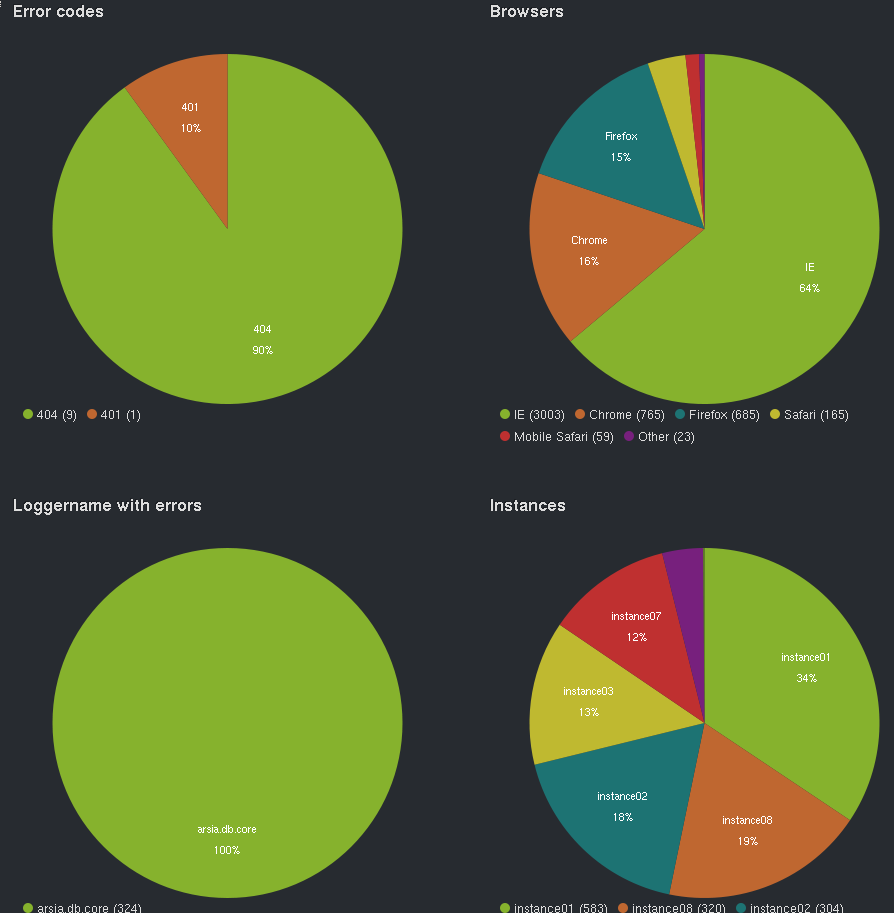
\includegraphics[height=7.5cm]{files/kibana3c.png}\\
    \end{center}
}
\frame{%
\frametitle{Kibana}
    \begin{center}
        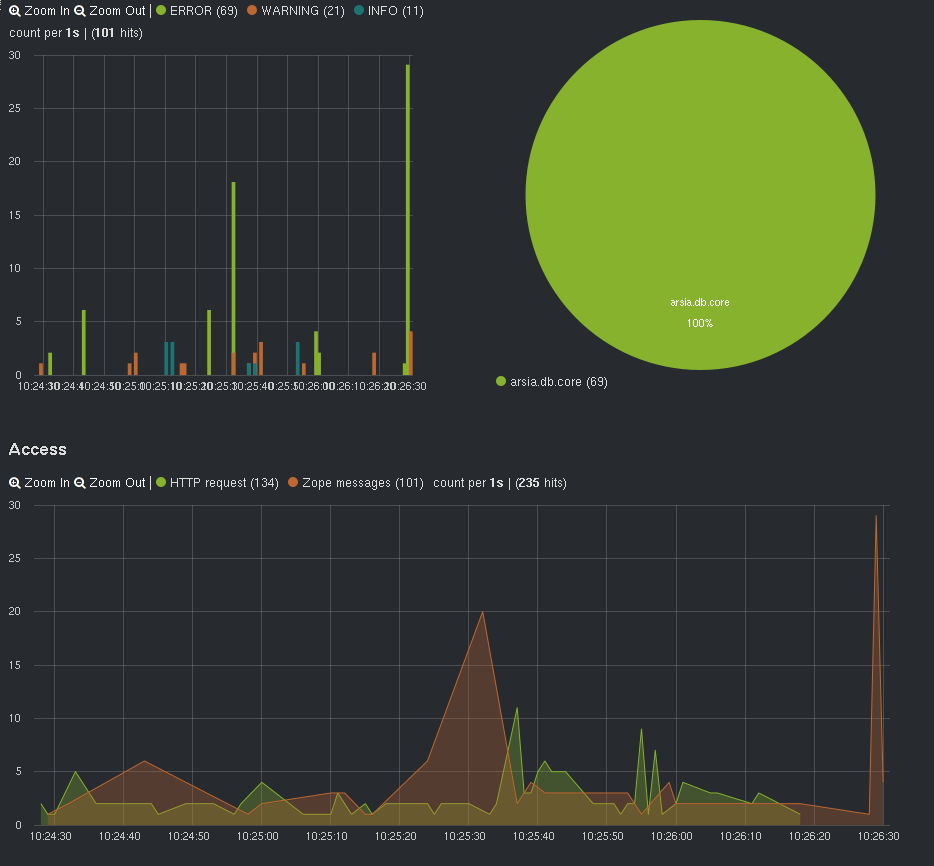
\includegraphics[height=7.5cm]{files/kibana3d.png}\\
    \end{center}
}
\section{Conclusion}
\frame{%
\frametitle{Conclusion}
\begin{itemize}
\xitem{Logstash is a small daemon}
\xitem{Simple to package \& deploy (jar file)}
\xitem{Scalable thanks to Elasticsearch}
\xitem{Developer friendly thanks to Kibana}
\end{itemize}
}



\end{document}
